\documentclass[10pt]{article}

\usepackage[utf8]{inputenc}

\usepackage[a4paper, portrait, left=2.25cm, right=2.25cm, top=2cm, bottom=2cm]{geometry}
\usepackage{graphicx, wrapfig}
\usepackage[toc,page]{appendix}
\graphicspath{ {./pictures} }

\title{Coursework 2 - interactive animated scene}
\author{Boyan Karatotev}
\date{}


\begin{document}
    \maketitle

    \section{Introduction}

        The scene for this coursework is the hedolar system in dimension
        42/$\aleph$. It has the ultimate icosahedron as a star, orbited by
        jellyfied Saturn and the spirits of the sages of this universe. From
        our home planet, orbiting Saturn, the BOSA (Bosnian Space Agency) is
        preparing for interstellar colonisation. We observe this solar system
        as one of the early explorers.


    \section{Basic building blocks}
        \begin{wrapfigure}{L}{0.2\textwidth}
            \caption{The rocket}
            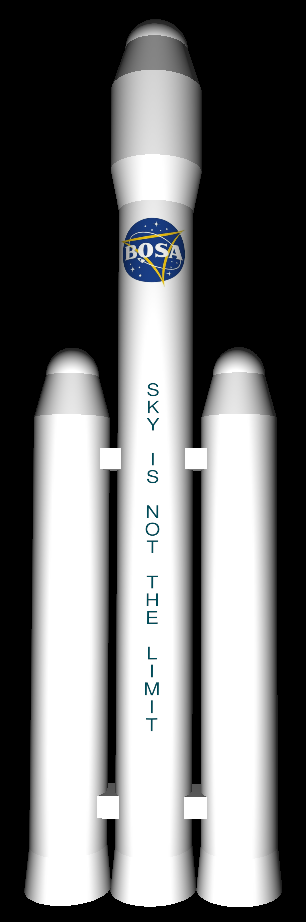
\includegraphics[width=0.2\textwidth]{rocket}
        \end{wrapfigure}


        For the convex object requirement there is an icosahedron. It is drawn
        by taking the coordinates of its 12 vertices and manually drawing the
        20 faces. Their values are not entirely hard-coded as normals are
        calculated from the vertices of each face. Extra care for the order of
        the vertices (counterclockwise) ensures they are always correct.

        Apart from the icosahedron, there is also a cube done manually by a
        different method, which was not used further as using gluQuadric for
        everything else was more convenient. This includes disks (with an
        option to have a hole), cylinders, spheres and frustums.

        All of these objects are of unit length (either radius or edge length).
        For correct dimensions they are scaled, rotated and translated instead
        of drawing them "properly". This makes texturing more complicated, as
        the object is the same shape and size as far as they are concerned. I
        came up with a workaround to scale and rotate the texture matrix to
        achieve the desired effect, although it did not end up being necessary.

        Material and texture properties are not set for any of them. It is the
        responsibility of the caller to set them up correctly. This worked
        quite well as it gave granular control for the different models.


    \section{The star}

        \begin{wrapfigure}{r}{0.2\textwidth}
            \caption{The star}
            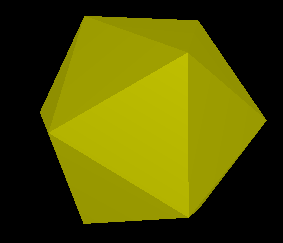
\includegraphics[width=0.2\textwidth]{star}
        \end{wrapfigure}

        The star in the hedolar system is an icosahedron, therefore the light
        source of the scene is at its centre. That means that every face has
        the light from directly behind it at all times and is unlit. To work
        around this, its emissivie light properties are set. However, it still
        looks wrong, as there is no diffusive or specular light to give it
        shades so it appears flat (yellow in this case). To combat this problem
        the scene has a second light with very low intensity at the camera. The
        reflectance of the icosahedron is set very high relative to the other
        objects so that the second light lights it brightly while not affecting
        the other objects much. It was an option to only enable the light while
        drawing the icosahedron, but having a small highligh on the backs of
        objects is a nice effect to distinguish them from the darkness of
        space.


    \section{The rocket}

        The rocket (the Heavy Large Aerial Delivery Automobile, HLADA) is a
        more highly advanced version of the only BOSA rocket flown to date (the
        Large Aerial Delivery Automobile, LADA). It is designed after the
        Falcon Heavy. It has three identical boosters made out of an elongated
        cylinder with conical frustums for engines capped with solid disks. The
        two side boosters have an aerodynamic top made out of a frustum and a
        cylinder. The middle booster is longer and has the second stage on top
        (frustum + cylinder) topped with the same cap as the other boosters.
        All three are connected by two struts on each side, made out of
        elongated cubes.

        All shapes use the same material properties. They have high diffusive
        reflecatance, somehwat low specular and is not particularly shiny so
        that it appears smooth but has a slighlty more accented highlight. The
        middle booster bears the BOSA logo, along with their slogan "Sky is not
        the limit", as a texture mapped with no distortion or repetition
        (although the setting is set to mirrored repeat). The different
        repeating parts (like the boosters) are instanced themselves to
        simplify the code.

        Although the rocket is a hierarchical model, it has no movement.


    \section{The planets}

        \begin{wrapfigure}{r}{0.5\textwidth}
                \caption{Marc}
                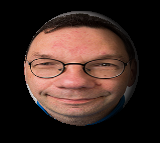
\includegraphics[width=0.2\textwidth]{marc}
                \caption{Marcus}
                \includegraphics[width=0.2\textwidth]{Marcus}
        \end{wrapfigure}

        There are four planets. All are textured generic spheres with smooth
        lighting. All orbit the star.

        The biggest one is textured as Saturn. It has its rings which are drawn
        as two disks with a hole in the middle. One of them is flipped so that
        it appears the same on both sides (I have culling of backs enables).
        Saturn's axis is tilted by the astronomically correct 26.73 degrees.
        Saturn and its satellites are meant to demonstrate hierarchical
        modelling with animation.

        Around it orbits another sphere textured as the Earth. It behaves
        essentially the same way, except that its orbit around Saturn is
        independent.

        On the Earth are placed 5 rockets to demonstrate instancing. They are
        on the equator, where every reasonable space exploring civilisation
        would place them. They are placed unmodified as described before,
        distanced equally apart. Admittedly, their size and placement is
        concerning for the tidal forces and the orbit of the planets. The
        Croatian scientists have repeatedly assured us that this will not be a
        problem when they launch.

        Finally, the two sages have an inner and an outer orbit relative to
        Saturn. They are spheres with the Marc and Marcus textures. They
        stretch somewhat oddly onto spheres but it looks reasonable.


        All plantes orbit around the star independently in their own orbits.


        \begin{figure}[h!]
            \caption{The Saturn system}
            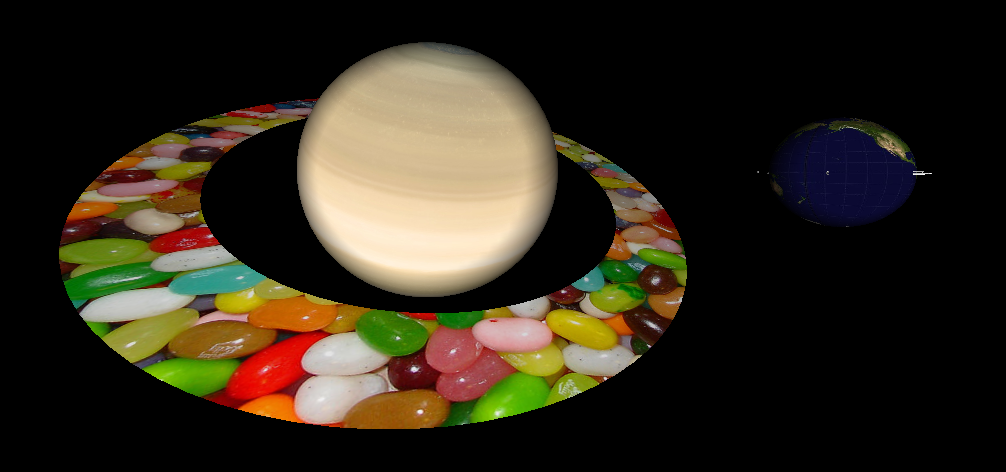
\includegraphics[width=\textwidth]{saturn_system}
        \end{figure}

    \pagebreak
    \section{User interaction}

        \begin{wrapfigure}{R}{0.2\textwidth}
            \caption{Control menu}
            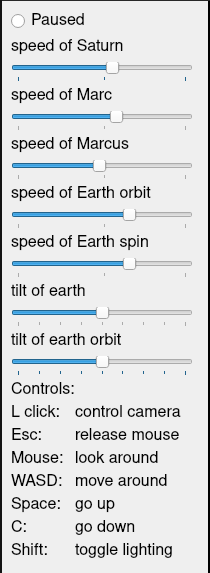
\includegraphics[width=0.2\textwidth]{controls}
        \end{wrapfigure}

        There are three forms of user interaction.

        First is by mouse. When the openGL widget is clicked, it captures the
        mouse and starts tracking it. Moving it rotates the camera in that direction.

        Second is by keyboard. the WASD keys move the camera in the direction
        it is facing. Space/C move it up/down in the y direciton only. Escape
        releases the mouse if captures and Shift toggles the lighting.

        Third is with Qt widgets. There are sliders in both positive and
        negative directios for most orbital parameters of the system, like
        speeds of orbits, speeds of rotation around an axis and angles of
        different axes. There is also a toggle for all movement via a radio
        button to more easily look around the scene.


    \begin{appendices}
        \section{The "I don't get the joke" part}

            It should be noted that I am neither Bosnian, nor does the BOSA
            actually exist. I am, however, from the Balkans which is good engough.
            This is meant to go with joke from "Space Song" by Dubioza Kolektiv,
            where the BOSA launches a LADA car/rocket into space, hence the
            acronym. HLADA furthers the pun, as in most eastern slavc languages it
            can mean "cold". Furthermore, Boza (written with a z, however) is a
            popular beverage in the Balkans.

            Everything else comes from the surreal meme "Riddle of the rocks" on
            the BagelBoy youtube channel.

            Finally, the "The Hitchhiker's Guide to the Galaxy" reference is
            mandatory. Bring a towel!

    \end{appendices}
\end{document}
